%Autor: miguev
%miguev: 24

\chapter{GNU R}
\label{r.tex}

\index{R}
\index{GNU R}

\section{Introducción}

%%%%%% Traducido de la web de R en http://www.r-project.org

{\sf R}  es a  la vez un  entorno y un  lenguaje de  programación para
realizar cálculos y gráficos estadísticos. Es un proyecto GNU similiar
al  sistema {\sf  S}  desarrollado en  Bell Laboratories  (formalmente
AT\&T, ahora  Lucent Technologies)  por John  Chambers y  sus colegas.
{\sf R} puede  considerarse como una implementación  diferente de {\sf
S}. Hay diferencias importantes entre ambos, pero mucho código escrito
para el sistema {\sf S} puede ejecutarse en {\sf R} sin modificarlo.

{\sf  R}  proporciona  una  amplia  variedad de  técnicas  gráficas  y
estadísticas (regresiones  lineales y no lineales,  tests estadísticos
clásicos, análisis  de series temporales,  clasifiaciones, clustering,
etc.)  y además  es  muy extensible.  El lenguaje  {\sf  S} suele  ser
utilizado para la investigación en  metodología estadística, y {\sf R}
proporciona una alternativa de código abierto para esta actividad.

Uno de  los puntos fuertes de  {\sf R} es  la facilidad con la  que se
pueden  producir  gráficas  de  buen diseño  y  calidad  de  imprenta,
incluyendo  símbolos y  fórmulas  matemáticas  donde sean  necesarias.
Aunque {\sf R}  pone un gran cuidado en las  opciones por defecto para
el diseño de las gráficas, el  usuario puede tener control total sobre
éstas.

{\sf R}  es Software  Libre, disponible  bajo los  términos de  la GNU
General Public  License de  la Free Software  Foundation, en  forma de
código fuente. Se puede compilar y  ejecutar en una amplia variedad de
plataformas  UNIX  (incluyendo  Linux  y  FreeBSD),  MacOS  y  Windows
9x/NT/2000.

El  código  fuente  de  {\sf  R} se  puede  descargar  del  sitio  web
del  proyecto {\sf  R} ({\tt  http://www.r-project.org}), así  como su
documentación. Además de la  documentación oficial (en inglés) existen
otros  documentos {\em  contribuidos} entre  los que  se encuentra  la
traducción  al  español  de  ``An Introduction  to  R''  y  ``Gráficos
Estadísticos con R''. \index{R!documentación}  Estos y más manuales se
encuentran en el CRAN (Comprehensive R Archive Network), concretamente
en {\tt http://cran.r-project.org/other-docs.html}

%%%%%%

\section{El entorno R}

\index{R!entorno}

{\sf  R} es  un conjunto  integrado de  utilidades para  manipulación,
cálculo  y  representación  de  datos.  Decimos  que  {\sf  R}  es  un
{\em entorno}  porque es  un sistema  diseñado para  ser completamente
coherente.  El  entorno  de   {\sf  R}  proporciona  facilidades  para
manipulación  y almacenamiento  de  datos,  operaciones con  variables
indexadas  (como vectores  y matrices),  análisis y  representación de
datos, un lenguaje de programación  bien desarrollado (con todo lo que
cabe esperar  de un lenguaje  de programación) y una  amplia colección
integrada y coherente de utilidades para análisis de datos.

Aunque mucha  gente utiliza {\sf  R} como un sistema  estadístico, sus
autores  prefieren considerarlo  como ``un  entorno en  el que  se han
implementado muchas  técnicas estadísticas, clásicas y  modernas''. La
mayoría  de la  estadística clásica  y muchas  de los  últimos métodos
están disponibles en  {\sf R}, aunque posiblemente  tendrás que buscar
un rato para encontrarlas.

La forma de trabajar  con {\sf R} es distinta a  la de otros programas
como {\tt SPSS}. En {\sf R}, un análisis estadístico se realiza en una
serie de pasos, con unos resultados intermedios que se van almacenando
en  objetos,   para  ser   observados  o   analizados  posteriormente,
produciendo unas salidas  mínimas. En {\tt SPSS} se  obtendría de modo
inmediato  una  salida copiosa  para  cualquier  análisis. Esto  puede
parecer a primera  vista una terrible incomodidad,  pero si tuviéramos
que  trabajar en  una máquina  poco potente  rápidamente nos  daríamos
cuenta de que puede resultar muy ventajosa la sencillez del entorno de
{\sf  R} (un  entorno de  comandos) y  la posibilidad  de ver  en cada
momento exactamente lo  que se necesita, sin  excesos que desperdicien
recursos del sistema.

Aún así, la mejor  manera de trabajar con R es  en un entorno gráfico,
con un sistema de ventanas como  X-Window, de forma que puedas ver las
gráficas en el momento de generarlas.

Veamos cómo se trabaja con {\sf  R} usándolo. En primer lugar conviene
crear un  directorio y entrar en  él antes de comenzar  una sesión con
{\sf  R}, que  en  éste almacena  siempre en  el  directorio donde  se
ejecutan unos ficheros donde almacena  los objetos, datos, funciones y
comandos ejecutados.  Esto puede sernos  muy útil en  trabajos largos,
podemos  interrumpir la  sesión con  {\sf  R} en  cualquier momento  y
recuperarla luego donde mismo la dejamos.

Hemos considerado a lo largo de  este curso que el símbolo del sistema
Linux/UNIX es  {\tt \$}. Vamos a  considerar ahora que el  símbolo del
prompt  {\sf R}  es {\tt  $>$}. \index{R!prompt}  Abre un  emulador de
terminal dentro del entorno gráfico y ejecuta los siguientes comandos:

\begin{verbatim}
$ mkdir sesion_R
$ cd sesion_R
$ R

R : Copyright 2002, The R Development Core Team
Version 1.5.1  (2002-06-17)

R is free software and comes with ABSOLUTELY NO WARRANTY.
You are welcome to redistribute it under certain conditions.
Type `license()' or `licence()' for distribution details.

R is a collaborative project with many contributors.
Type `contributors()' for more information.

Type `demo()' for some demos, `help()' for on-line help, or
`help.start()' for a HTML browser interface to help.
Type `q()' to quit R.

> 
\end{verbatim}

El prompt de {\sf R} indica  el entorno que está esperando tus órdenes
para ejecutarlas. Para salir del entorno de {\sf R} puedes utilizar la
función {\tt q()}  o pulsar {\tt C-d}, entonces {\sf  R} te preguntará
si  deseas  guardar el  {\em  espacio  de  trabajo},  que es  toda  la
información sobre la sesión que quieres cerrar:

\index{R!sesiones}

\begin{verbatim}
> q()
Save workspace image? [y/n/c]: 
\end{verbatim}

Para salir guardando la sesión pulsa {\tt y}, para salir sin guardarla
pulsa {\tt n} y para para cancelar la salida pulsa {\tt c}. Si guardas
la  sesión al  salir quedará  almacenada en  el directorio  en el  que
ejecutaste {\tt R},  y será automáticamente recuperada  la próxima vez
que ejecutes {\tt R} dentro del directorio en cuestión.

{\sf R} dispone de un sistema de ayuda similar a las páginas de manual
de  Linux/UNIX. Cuando  necesites información  sobre una  función, por
ejemplo {\tt  solve}, ejecuta la  función {\tt help()}  pasándole como
parámetro el nombre de la función que quieras consultar. También existe
una forma más corta: {\tt ?función}:

\index{R!ayuda}
\index{R!help@{\tt help()}}

\begin{verbatim}
> help (solve)
> ?solve 
\end{verbatim}

Normalmente  puedes  ver  la  documentación también  en  el  navegador
web. Si  ejecutas {\tt  help.start()} debería  abrirse una  ventana de
navegador  con la  documentación en  formato HTML  por la  cual puedes
navegar para buscar lo que necesites.

Otra forma muy interesante de buscar  ayuda dentro del entorno de {\sf
R}  es pasarle  una  palabra  a la  función  {\tt help.search()}.  Por
ejemplo, para buscar  una función que resuelva  sistemas de ecuaciones
puedes empezar por buscar la palabra {\tt solve}.

\index{R!búsqueda}
\index{R!help.search@{\tt help.search()}}

\begin{verbatim}
> help.search ("solve")

Help files with alias or title matching `solve',
type `help(FOO, package = PKG)' to inspect entry `FOO(PKG) TITLE':

backsolve(base)         Solve an Upper or Lower Triangular System
qr(base)                The QR Decomposition of a Matrix
solve(base)             Solve a System of Equations
\end{verbatim}

De un  primer golpe  ya sabes  que el  paquete {\tt  base} de  {\sf R}
tiene  funciones para  resolver  sistemas  triangulares (superiores  o
inferiores), descomponer matrices  en la forma QR  y resolver sistemas
de ecuaciones (cualesquiera).

{\sf  R} proporciona  algunas  demostraciones  sobre sus  capacidades.
Para  ir abriendo  el apetito  ejecuta la  funciones que  muestran las
demostraciones con gráficos e imágenes:

\begin{verbatim}
> demo (graphics)
> demo (images)
\end{verbatim}

%\begin{figure}[hbtp]
%\centering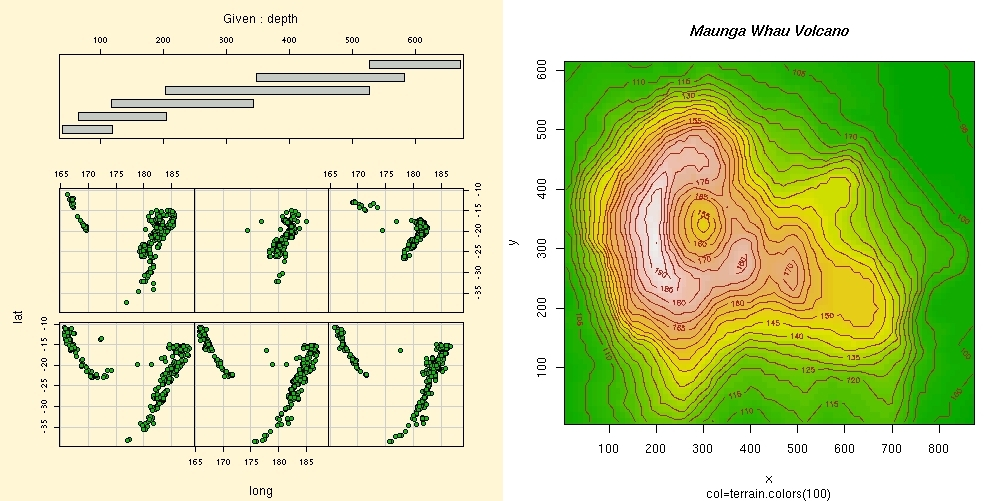
\includegraphics[width=\textwidth]{imagenes/r_demos.eps}
%\index{R!demos}
%Demostraciones sobre gráficos e imágenes
%\end{figure}

\begin{figura}{r_demos}{1}
\index{R!demos}
\caption{Demostraciones sobre gráficos e imágenes}
\end{figura}


\section{El lenguaje {\sf R}}

\index{R!lenguaje}

{\sf R} es también lenguaje de  programación en toda regla, con el que
puedes escribir  programas que  procesen ficheros  de datos  y generen
análisis y representaciones de los datos.

Al igual que  la mayoría de lenguajes basados en  UNIX, el lenguaje de
{\sf R} distingue entre mayúsculas y minúsculas. Esto es, {\tt esto} y
{\tt  Esto} son  símbolos  distintos y  pueden  referirse a  variables
distintas. En {\sf  R} los nombres de variables pueden  tener letras y
números  (como en  casi cualquier  lenguaje), aunque  {\bf no}  pueden
tener el  subrayado ({\tt \_}),  pero en su  lugar sí pueden  tener el
punto.  De hecho  se suele  utilizar  el punto  para separar  palabras
en  los  nombres  de  las  variables en  {\sf  R},  por  ejemplo  {\tt
hoja.de.datos}.

\index{R!órdenes}
\index{R!comandos}

Las órdenes  (o comandos) elementales son  expresiones o asignaciones.
Si ejecutas  una expresión como comando  ésta se evalúa y  se imprime,
pero su valor se pierde. En una asignación la expresión se evalúa y su
valor se almacena en la varbiable, pero no se imprime.

Los comandos se  separan con el caracter  de punto y coma  ({\tt ;}) o
simplemente  con una  salto  de  línea. Puedes  agrupar  una serie  de
comandos  encerrándolos entre  llaves,  de esta  forma puedes  definir
funciones como veremos más adelante. También puedes poner comantarios,
\index{R!comentarios} casi  donde quieras\footnote{No puedes  meter un
comentario dentro  de una cadena  de caracteres (formaría parte  de la
cadena), ni en medio de la lista de argumentos en la definición de una
función}, poniendo  una almohadilla ({\tt \#})  y todo lo que  la siga
hasta el final de línea será obviado por el intérprete de {\sf R}.

Si dejas  un comando a medias  {\sf R} se  dará cuenta, y en  lugar de
mostrarte el prompt  $>$ te mostará {\tt +} para  avisarte de que está
esperando por el final del comando.

Otra característica  interesante de {\sf  R} (al menos  en plataformas
Linux/UNIX)  es  la  posibilidad  de  editar  la  línea  de  comandos.
Esto  incluye  el  típico  historial   de  comandos,  que  te  permite
repetir  los comandos  sin tener  que  volver a  teclearlos. Tan  solo
utiliza los  cursores arriba y  abajo para recuperar los  comandos que
hayas tecleado.  \index{R!historial} Además este historial  de comando
queda  almacenado en  la  sesión  cuando sales  del  entorno {\sf  R},
concretamente en  un fichero  {\tt .Rhistory}  en el  directorio donde
ejecutaste en entorno {\sf R}.

Pero si necesitas usar una serie un poco larga de comandos seguramente
te canses de tener  que darle a los cursores. Para  estos casos lo que
necesitas  es un  script en  el que  escribes los  comandos a  modo de
programa. Luego para ejecutar los  comandos escritos en él utilizas la
función {\tt  source ()} del  entorno pasándole el nombre  del fichero
donde escribiste los comandos:

\index{R!leer comandos de un fichero}
\index{R!source@{\tt source()}}

\begin{verbatim}

> source ("script.R")

\end{verbatim}

Del  mismo modo  que puedes  tomar la  entrada de  un fichero  también
puedes redireccionar la salida hacia otro fichero, con la función {\tt
sink()}. Para almacenar la salida en el fichero {\tt salida.txt} 
ejecuta el comando:

\index{R!volcar en un fichero}
\index{R!sink@{\tt sink()}}

\begin{verbatim}

> sink ("salida.txt")

\end{verbatim}

Para devolver  la salida al  intérprete utiliza la misma  función {\tt
sink  ()}  pero sin  pasarle  ningún  parámetro.  En el  fichero  {\tt
iodemo.R}  tienes un  ejemplo de  esto. 

\begin{ejemplo}{iodemo.R}{Uso de {\tt sink()}}
Este script lee  una tabla que está almacenada en  un fichero de texto
llano ({\tt muestra.dat}, que usaremos para los ejemplos) y extrae dos
variables  de ella.  Para  ambas variables  muestra  un breve  resumen
estadístico, pero guarda uno en el  fichero {\tt salida.txt} y el otro
lo muestra en el entorno {\sf R}.
\end{ejemplo}

Entra en el directorio donde tengas el fichero y ejecuta en el entorno
{\sf R}

\begin{verbatim}
> source ("iodemo.R")
\end{verbatim}

\section{Vectores}

\index{R!vectores}

{\sf R} realiza las operaciones sobre las llamadas {\em estructuras de
datos}, de las cuales la más  simple es el vector numérico. Para crear
un vector con  los 5 primeros números enteros  positivos utilizamos la
función {\tt  c()} que  combina los objetos  recibidos para  formas un
vector:

\begin{verbatim}
> x <- c (1, 2, 3, 4, 5)
> x
[1] 1 2 3 4 5
\end{verbatim}

\index{R!asignación, operador de}

En efecto, el operador de asignación no se parece para nada a un signo
de igualdad. De  hecho es una flecha, que está  indicando que el valor
de lo que hay a su derecha debe asignarse a lo que hay a su izquierda.
Si le das la vuelta a la flecha funciona al revés:

\begin{verbatim}
> c (6, 7, 8, 9, 10) -> y
> y
[1]  6  7  8  9 10
\end{verbatim}

Cuando  ejecutas  el  nombre  de  un  objeto  como  comando,  {\sf  R}
interpreta que deseas  ver su contenido y entonces  ejecuta la función
{\tt print()} sobre  el objeto en cuestión. Esto  funciona sólo cuando
estás  dentro del  entorno {\sf  R} y  tecleas el  nombre del  objeto.
\index{R!print@{\tt print()}}
Cuando quieras imprimir  el objeto desde un fichero  de comandos (como
hacemos en {\tt iodemo.R}) has de utilizar la función {\tt print()}.

Dado que la función {\tt c()} combina objetos para formar vectores, 
también puede combinar varios vectores para formar un nuevo vector
que es el resultado de concatenar los anteriores:

\begin{verbatim}
> z <- c (x, y)
> z
 [1]  1  2  3  4  5  6  7  8  9 10
\end{verbatim}

Las  operaciones  usuales  entre  vectores  se  definen  ``elemento  a
elemento'':

\index{R!vectores!operaciones elementales}

\begin{verbatim}
> x + 2
[1] 3 4 5 6 7
> 2 * x
[1]  2  4  6  8 10
> x + y
[1]  7  9 11 13 15
> x - y
[1] -5 -5 -5 -5 -5
> x * y
[1]  6 14 24 36 50
> x / y
[1] 0.1666667 0.2857143 0.3750000 0.4444444 0.5000000
> y / x
[1] 6.000000 3.500000 2.666667 2.250000 2.000000
> x ^ y
[1]       1     128    6561  262144 9765625
> y ^ x
[1]      6     49    512   6561 100000
\end{verbatim}

Pero  entonces ¿cómo  se multiplican  escalarmente dos  vectores? Para
esto hay una función llamada  {\tt crossprod}, que permite multiplicar
dos  vectores  (o  matrices).  El operador  \verb|%*%|  es  una  forma
abreviada  de  este  producto.  Formalmente  {\tt  crossprod(x,y)}  es
equivalente a  {\tt t(x) \%*\%  y}, pero  más rápido. La  función {\tt
t()} es la trasposición de matrices:

\index{R!vectores!producto escalar}

\begin{verbatim}
> x
[1] 1 2 3 4
> y
[1] 4 5 6 7
> crossprod(x,y)
     [,1]
[1,]   60
> x %*% y
     [,1]
[1,]   60
\end{verbatim}

Además de para guardar datos,  los vectores suelen usarse para definir
series o  secuencias. Para  definir una  secuencia de  números enteros
consecutivos basta  con poner el primer  y el último separados  por un
caracter de dos puntos:

\index{R!vectores!secuencias}

\begin{verbatim}
> x <- 1:10
> x   
 [1]  1  2  3  4  5  6  7  8  9 10
\end{verbatim}

Pero  para  generar   secuencias  la  mejor  manera   es  utilizar  la
función {\tt  seq()}. Si  le pasas tres  valores numéricos  le estarás
especificando el  primer y el  último elemento  de la secuencia,  y la
diferencia que debe haber entre cada dos elementos consecutivos:

\begin{verbatim}
> y <- seq (-1, 1, .2)
> y
 [1] -1.0 -0.8 -0.6 -0.4 -0.2  0.0  0.2  0.4  0.6  0.8  1.0
\end{verbatim}

Para replicar  un objeto  varias veces, por  ejemplo para  generar una
secuencia  periódica,  utiliza la  función  {\tt  rep()} pasándole  el
objeto y el número de veces que quieres replicarlo:

\begin{verbatim}
> z <- rep (seq (-1, 1, 1), 5)
> z
 [1] -1  0  1 -1  0  1 -1  0  1 -1  0  1 -1  0  1
\end{verbatim}

Además de vectores numéricos, {\sf R} permite operar con vectores {\em
lógicos}.  Los valores  válidos  para los  elementos  de los  vectores
\index{R!vectores!vectores lógicos}
lógicos son los de la {\em lógica  triestada}: 
\index{lógica triestada}
{\tt TRUE}, {\tt FALSE} y {\tt NA} (``Not Available'', no disponible).
Los operadores  lógicos para manejar  estos valores son {\tt  \&} para
``and'', {\tt |} para ``or'' y {\tt !} para ``not''.

Una forma  de generar  un vector  de valores  lógicos es  efectuar una
comparación entre un vector numérico y un valor numérico:

\begin{verbatim}
> z <- rep (seq (-1, 1, 1), 3)
> z
[1] -1  0  1 -1  0  1 -1  0  1
> z > 0
[1] FALSE FALSE  TRUE FALSE FALSE  TRUE FALSE FALSE  TRUE
\end{verbatim}

Al contrario que  en la mayoría de lenguajes de  programación, en {\sf
R}  los vectores  se indexan  comenzando por  $1$. Para  acceder a  un
elemento  de un  vector utiliza  la notación  usual de  los corchetes.
También puedes acceder a un  subconjunto del vector especificando como
índice un vector con las posiciones de los elemenos:

\index{R!vectores!índices}
\index{R!vectores!subíndices}
\index{R!vectores!indixado}

\begin{verbatim}
> x <- 1:10
> x
 [1]  1  2  3  4  5  6  7  8  9 10
> x[2:5]
[1] 2 3 4 5
> x[8:2]
[1] 8 7 6 5 4 3 2
\end{verbatim}

También puedes  acceder a  un subconjunto de  un vector  utilizando un
vector lógico:

\begin{verbatim}
> x[x > 4]
[1]  5  6  7  8  9 10
\end{verbatim}

Incluso puedes indexar  un vector no palabras, poniendo  nombres a las
posiciones dentro del vector mediante  la función {\tt names()}. Luego
puedes acceder a los elementos mediante los nombres de las posiciones:

\index{R!vectores!nombres}
\index{R!vectores!names@{\tt names()}}

\begin{verbatim}
fruta = c (5, 10, 1, 20)
> fruta <- c (5, 10, 1, 20)
> names (fruta) <- c ("naranja", "plátano", "manzana", "ñame")
> fruta[c ("manzana", "naranja")]
manzana naranja 
      1       5 
> fruta
naranja plátano manzana    ñame 
      5      10       1      20 
\end{verbatim}

\section{Arrays y matrices}

\index{R!arrays}
\index{R!matrices}

Un   {\em   array}\footnote{a   veces   traducido   por   ``arreglo''}
\index{arreglo} es  una variable indexada multidimensional.  Un vector
es un  array unidimensional  y una matriz  es un  array bidimensional.
{\sf R} proporciona un buen manejo de arrays, sobretodo para matrices.

La dimensión de un array es un vector cuya longitud es la dimesión del
array,  y  cada uno  de  sus  elementos  es  la ``longitud''  de  cada
dimensión en el array. Por  ejemplo, un array con dimesión $(3,5,100)$
sería como un cubo de $1500$ elementos con $3$ celdas de largo, $5$ de
ancho y $100$ de alto.

\index{R!arrays!dimensión}

En la  mayoría de  lenguajes los  elementos de  un array  se almacenan
``por filas'', lo que significa que el índice que avanza más rápido es
el último. Sin embargo, en {\sf R}  la ordenación se hace al estilo de
FORTRAN, ordenando  los elementos  ``por columnas'', lo  que significa
que el índice que avanza más rápido es el primero.

Es importante tener esto en cuenta porque a la hora de crear una 
matriz hay que proporcionar los elementos agrupados por columnas, no 
por filas. Por ejemplo:

\index{R!arrays!por filas}
\index{R!arrays!por columnas}


\begin{verbatim}
> a <- array (c (1:3,-3:-1), dim = c (3,2)) 
> a
     [,1] [,2]
[1,]    1   -3
[2,]    2   -2
[3,]    3   -1
\end{verbatim}

Para  acceder a  los elementos  de una  matriz (o  array) ponemos  los
subíndices  entre corchetes  y  separados por  comas.  Si omitimos  el
subíndice de las filas (el  primero) obtenemos la columna señalada por
el segundo subíndice, y análogamente  obtenemos las filas omitiendo el
segundo suníndice.

\index{R!arrays!índices}
\index{R!arrays!subíndices}
\index{R!arrays!indexado}

\begin{verbatim}
> a[1,2]
[1] -3
> a[,2]
[1] -3 -2 -1
> a[1,]
[1]  1 -3
\end{verbatim}

De la misma forma que podemos extraer elementos, filas o columnas de
una matriz también podemos asignarles valores:

\begin{verbatim}
> a[,2] <- 3:5
> a[,2]
[1] 3 4 5
> a
     [,1] [,2]
[1,]    1    3
[2,]    2    4
[3,]    3    5
\end{verbatim}

Para multiplicar  matrices (o arrays  en general) utiliza  el operador
\verb|%*%| que vimos antes:

\index{R!arrays!producto}
\index{R!matrices!multiplicar}

\begin{verbatim}
> a
     [,1] [,2]
[1,]    1    3
[2,]    2    4
[3,]    3    5
> b = array (1:2, 2:1, dim = c (2,2))
> b
     [,1] [,2]
[1,]    1    1
[2,]    2    2
> a %*% b
     [,1] [,2]
[1,]    7    7
[2,]   10   10
[3,]   13   13
\end{verbatim}

Vimos antes  que si multiplicamos dos  vectores {\tt x} y  {\tt y} (de
igual longitud) utilizando el operador  {\tt \%*\%} el resultado es el
producto  escalar de  los vectores.  En realidad  la operación  {\tt x
\%*\%  y}  es ambigua,  porque  podría  significar  $x'  x$ o  $x  x'$
(considerando $x$ un vector columna).  En estos casos de ambigûedad se
considera implícitamente  que la interpretación deseada  es aquella de
la  que resulte  la  matriz más  paqueña,  por lo  que  se obtiene  el
producto escalar $x' x$.

Para  calcular la  matriz $x  x'$ puedes  utilizar las  funciones {\tt
cbind()} y {\tt rbind()}, ya que éstas siempre devuelven matrices. Las
funciones {\tt  cbind} y  {\tt rbind}  toman una  serie de  vectores o
números y los agrupan por columnas o filas en una matriz.

\index{R!matrices!cbind@{\tt cbind()}}
\index{R!matrices!rbind@{\tt rbind()}}

\begin{verbatim}
> x
[1] 1 2 3 4
> y
[1] 4 5 6 7
> x %*% y
     [,1]
[1,]   60
> cbind(x,y)
     x y
[1,] 1 4
[2,] 2 5
[3,] 3 6
[4,] 4 7
> rbind(x,y)
  [,1] [,2] [,3] [,4]
x    1    2    3    4
y    4    5    6    7
> cbind(x) %*% rbind(y)
      
       [,1] [,2] [,3] [,4]
  [1,]    4    5    6    7
  [2,]    8   10   12   14
  [3,]   12   15   18   21
  [4,]   16   20   24   28
\end{verbatim}


\section{Factores: clasificación de datos}

\index{R!factores}
\index{R!clasificación de datos}

Un  {\em factor}  es un  vector  que utilizamos  para especificar  una
clasificación  discreta (agrupamiento)  de  los  componentes de  otros
vectores del mismo tamaño. Para entender  lo que son los factores nada
mejor que un ejemplo claro y sencillo. En el entorno {\sf R} y ejecuta
lo siguiente:

\begin{verbatim}
> edad <- c (13, 16, 15, 17, 17, 18, 16, 16, 15, 16)
> sexo <- c ("hombre", "hombre", "mujer", "hombre", "mujer", "mujer",         
+            "hombre", "mujer", "hombre", "mujer") 
> edad
 [1] 13 16 15 17 17 18 16 16 15 16
> sexo
[1] "hombre" "hombre" "mujer"  "hombre" "mujer"  "mujer"  "hombre" 
[9] "mujer" "hombre" "mujer"
\end{verbatim}

Ahora tienes  una variable {\tt  edad} que  contiene las edades  de 10
personas, y  una variable {\tt  sexo} que define  el sexo de  cada una
de  las  10  personas  anteriores  (en el  mismo  orden)  y  que  toma
únicamente  los  valores  \verb|"hombre"| y  \verb|"mujer"|.  Vamos  a
calcular  la media  y  la  varianza muestrales  de  la  edad de  estas
personas  clasificándolas según  el sexo,  i.e. la  edad media  de los
hombres por un lado y la de las mujeres por otro.

Necesitamos  separar (agrupar)  los  elementos del  vector {\tt  edad}
según los valores que toma el  vector {\tt sexo}. Para esto utilizamos
un factor.  El factor  en realidad  es como  el vector  original, pero
tiene un atributo  añadido llamado {\tt levels} (niveles)  que son los
distintos  valores que  toman los  elementos del  vector original.  En
el  caso del  vector  {\tt  sexo} los  niveles  son \verb|"hombre"|  y
\verb|"mujer"|. La función  {\tt levels} devuelve la  lista de niveles
que tenga el factor que le pases como parámetro.

\begin{verbatim}
> sexo.factor = factor (sexo)
> sexo.factor
[1] hombre hombre mujer  hombre mujer  mujer  hombre mujer  hombre
Levels:  hombre mujer 
> levels (sexo.factor)
[1] "hombre" "mujer"
\end{verbatim}

Ahora queremos  aplicar unas  funciones, en este  caso {\tt  mean()} y
{\tt  var()}, a  un  vector de  datos  de manera  que  los datos  sean
separados según  un factor.  La función apropiada  para esta  tarea es
{\tt tapply}, y se usa del siguiente modo:

\index{R!tapply@{\tt tapply()}}

\begin{verbatim}
> tapply (edad, sexo.factor, mean)
hombre  mujer 
  15.4   16.4 
> tapply (edad, sexo.factor, var)
hombre  mujer 
   2.3    1.3
\end{verbatim}

Así obtenemos que dentro de esta muestra de 10 personas, la edad media
de los hombres es $15.4$ y  la de las mujeres $16.4$. Volveremos sobre
los factores más adelante, así que asegúrate de entender al menos este
uso de los mismos. Para mayores detalles consulta la ayuda de {\sf R}.

\section{Listas}

\index{R!listas}

En un  array todos  los elementos  deben ser del  mismo tipo,  i.e. no
puede  ser que  un array  contenga a  la vez  números y  palabras. Sin
embargo la  mayoría de muestras  contienen datos de  diferentes tipos:
números, palabras, valores lógicos, intervalos, etc.

Una {\em  lista} en {\sf  R} es una  colección ordenada de  objetos de
cualquier tipo. Es  como un vector, pero con la  diferencia de que sus
elementos pueden ser de distintos tipos. 

Los elementos de una lista están  siempre numerados por un subíndice y
puedes referirte  a ellos  como con un  vector, pero  usando corquetes
dobles.  Así  si {\tt  L}  es  una lista  {\tt  L[[1]]}  es su  primer
elemento. Pero también,  al igual que en los  vectores, puedes indexar
los elementos  de una lista dándoles  nombres. En caso de  nombrar los
elementos de una lista hay una  forma más cómoda de referirse a ellos:
en lugar de {\tt L[["nombre"]]} puedes usar {\tt L\$nombre}.

\index{R!listas!índices}
\index{R!listas!nombres}

\begin{verbatim}
> L = list (nombre = "Pepe", esposa = "Pepa", hijos = 3,
+     edades.hijos = c (34,6,12))
> L
$nombre
[1] "Pepe"

$esposa
[1] "Pepa"

$hijos
[1] 3

$edades.hijos
[1] 34  6 12

> L[["nombre"]]
[1] "Pepe"
> L$nombre
[1] "Pepe"
\end{verbatim}

Para concatenar  listas recuerda que  la función {\tt c()}  sirve para
ello.

\section{Hojas de datos}

\index{R!tablas}
\index{R!data frame}
\index{R!frame}
\index{R!hojas de datos}

Una ``hoja  de datos'' (en  inglés ``data frame'') es  básicamente una
lista de vectores, con algunas restricciones. Los vectores de palabras
son convertidos en factores.

Piensa en una hoja  de datos como su nombre sugiere:  una hoja o tabla
en la que tienes varios datos sobre varios individuos. Las columnas de
la hoja de  datos son los vectores  que la format, y cada  fila es una
lista.

En el  fichero {\tt  muestra.dat} tienes una  hoja de  datos preparada
para ser leida con la función  {\tt read.table()}. La primera fila son
los nombres  de los vectores columna,  y luego cada línea  del fichero
introduce  una lista  de  valores,  un valor  para  cada vector.  Para
entender esto con claridad lee  la tabla del fichero {\tt muestra.dat}
y mantenla en una variable:

\index{R!hojas de datos!leer desde fichero}
\index{R!read.table@{\tt read.table()}}

\begin{verbatim}
> hoja.de.datos = read.table ("muestra.dat") 
> names (hoja.de.datos)
[1] "Sexo"     "Edad"     "Habitat"  "Ingresos" "Lectura"  "TV"
\end{verbatim}

Esta tabla contiene  los datos (ficticios) de 50 jóvenes:  su sexo, su
edad,  su  hábidat,  sus  ingresos familiares  (en  miles  de  pesetas
mensuales),  el número  de libros  leidos  anualmente y  sus horas  de
televisión diarias.

Normalmente para  acceder al  vector {\tt  Edad} de  la hoja  de datos
utilizaríamos la expresión {\tt  hoja.de.datos\$Edad}, pero hay una forma
más cómoda. Consiste en ``conectar'' la hoja de datos para que puedas
referirte a sus vectores directamente por su nombre:

\index{R!hojas de datos!conectar}

\begin{verbatim}
> attach (hoja.de.datos)
> summary (Edad)
   Min. 1st Qu.  Median    Mean 3rd Qu.    Max. 
  12.00   15.00   16.00   15.64   17.00   20.00
\end{verbatim}

Ten en cuenta que  este atajo es sólo para {\em leer}  los datos de la
hoja, no para modificarlos. Si quieres  modificar un vector de la hoja
de datos tienes que usar la notación normal:

\begin{verbatim}
> hoja.de.datos$Edad <- Edad + 10
\end{verbatim}

De hecho, esto modifica  el vector en la hoja de  datos, pero no verás
los cambios en los atajos hasta que  desconectes la hoja de datos y la
vuelvas  a conectar.  Para desconectar  una hoja  de datos  utiliza la
función {\tt detach()}.

\index{R!hojas de datos!desconectar}

Cuando quieras  almacenar una hoja de  datos en un fichero  utiliza la
función {\tt write.table()}. Su uso básico es darle la hoja de datos y
el nombre del  fichero, pero admite varias  opciones para personalizar
la  forma en  la  que escribirá  los  datos en  el  fichero. Para  ver
estos  detalles consulta  la ayuda  sobre la  función ejecutando  {\tt
?write.table}. \index{R!hojas de datos!escribir en fichero}

\subsection{Valores perdidos}

\index{R!valores perdidos}

En ocasiones  te encontrarás  con hojas de datos  en las  que alguna
celda no tiene el dato. Esto puede suceder porque no haya sido posible
averiguar el dato,  o porque éste no tenga sentido.  En estos casos se
utiliza para esa  celda el valor {\tt NA}, que  significa que el valor
``no está disponible'' (NA es abreviatura de ``Not Available'').

\index{R!NA@{\tt NA}}

En otros casos sucede que tras efectuar una serie de operaciones sobre
un  conjunto de  datos algunos  de  los resultados  no tengan  sentido
matemático, como  por ejemplo una  división por cero (recuerda  que la
precisión  de los  procesadores es  limitada).  En caso  de hacer  una
operación así {\sf R} no se quejará en absoluto, sino que devolverá el
valor {\tt  NaN} que  significa que  eso ``no es  un número''  (NaN es
abreviatura de ``Not a Number'').

\index{R!NaN@{\tt NaN}}

\section{Funciones}

\index{R!funciones}

Como todo  buen lenguaje de  programación, {\sf R} te  permite definir
funciones  para tu  uso propio.  Para definir  una función  asignas al
objeto (que  será tu función)  el valor  devuelto por la  función {\tt
function}. Esta  función particular  recibe los mismos  parámetros que
recibirá  tu  función,  y  a  continuación  una  {\em  agrupación}  de
comandos, encerrados entre llaves y separados  con {\tt ;} o saltos de
línea. El  valor devuelto por  tu función será  el valor de  la última
expresión de la agrupación.

Por ejemplo  si quieres  una función  que calcule  la curtosis  de una
muestra:

\begin{verbatim}
> curtosis <- function (x) {
+ n <- length (x)
+ c <- ( (n * (n - 1) * sum((x - mean(x))^4) ) /
+      ( (n - 1) * (n - 2) * (n - 3) * (var(x))^4 ) ) -
+      ( (3 * (n - 1)^2) / ( (n - 2) * (n - 3) ) )
+ c 
+ }
> hoja.de.datos = read.table ("muestra.dat")
> attach (hoja.de.datos)
> curtosis (Edad)
[1] -2.921993
> curtosis (Lectura)
[1] -3.191575
> curtosis (TV)
[1] -3.192770
\end{verbatim}

Normalmente las funciones no quedan bien escritas a la primera, por lo
que tendrás que corregirlas una y  otra vez. O tal vez quieras definir
más funciones,  modificar las que  ya tengas escritas, etc.  Todo esto
puedes hacerlo más cómodamente si escribes las funciones en un fichero
y lo importas con la función {\tt source()} que vimos antes.

\index{R!funciones!leer desde fichero}

Así por ejemplo tienes escrita la función {\tt curtosis} en el fichero
{\tt curtosis.R}. Si quieres modificarla  y volver a usarla después de
modificada no  hay problema.  Edita el  fichero {\tt  curtosis.R} para
modificar la función  y luego vuelve a importarlo con  la función {\tt
curtosis}. Recuerda que la función {\tt source()} ejecuta los comandos
que encuentra en el fichero que le digas, por lo que las funciones que
tengas escritas en  el fichero serán redefinidas y  estarán lista para
usar al instante.

\begin{ejemplo}{curtosis.R}{Fichero de funciones}
Este fichero contiene la definición de  una función, y cada vez que lo
leas con  la función {\tt source()}  será ejecutado. Por lo  tanto las
funciones que  contiene son redefinidas,  lo que te  permite modificar
las funciones  y hacer efectivos los  cambios sin tener que  salir del
entorno.
\end{ejemplo}

\subsection{Control de flujo}

\index{R!funciones!control de flujo}

{\sf R} proporciona la sintaxis necesaria para construir funciones que
mantengan  en control  del flujo  del  programa. Nos  referimos a  los
condicionales y los bucles:

\subsubsection*{Ejecución condicional}

\index{R!funciones!if@{\tt if}}

La  forma  de  contruir  una  sentencia  condicional  en  {\sf  R}  es
{\tt  if (expresion\_logica)  sentencia\_1 else  sentencia\_2}. Si  la
{\tt  expresion\_logica}  es  cierta  (su  valor  es  {\tt  TRUE})  se
ejecutará la  {\tt sentencia\_1},  en otro caso  se ejecutará  la {\tt
sentencia\_2}.  {\tt sentencia\_1}  y  {\tt  sentencia\_2} pueden  ser
también agrupaciones de comandos y/o expresiones.

\begin{verbatim}
> x = 1      
> y = 2
> if (x > y) x else y
[1] 2
\end{verbatim}

En las  expresiones booleanas  puedes emplear  los operadores  {\tt |}
(OR) {\tt \&}  (AND) y {\tt !} (NOT) normales,  o si prefieres ahorrar
un poco de  tiempo los operadores ``cortocicuitados'' {\tt  ||} (OR) y
{\tt  \&\&}.  \index{R!||@{\tt  ||}} \index{R!\&\&@{\tt  \&\&}}  Estos
operadores lógicos  tienen la ventaja  de que sólo evalúan  la segunda
expresión cuando es necesario.

Para las  comparaciones numéricas se utilizan  los mismos comparadores
binarios que en el lenguaje C:  {\tt $<$}, {\tt $>$}, {\tt $<=$}, {\tt
$>=$}, {\tt  !=} y {\tt  ==}. Ten cuidado  de no utilizar  el operador
{\tt =} para comparaciones.

\index{R!funciones!ifelse@{\tt ifelse()}}

Existe  además  una  versión   {\em  vectorizada}  de  la  construción
condicional. Se trata  de la función {\tt ifelse ()},  que recibe tres
vectores {\tt condicion, a, b} y devuelve un vector del tamaño del más
largo.  En este  vector  el  elemnto i-ésimo  es  {\tt  a[i]} si  {\tt
condicion[i]} es cierto (su valor es {\tt TRUE}) o bien {\tt b[i]}) en
caso contrario.

\begin{verbatim}
> condicion = c (TRUE, FALSE)
> a = c (1, 2)
> b = c (3, 4)
> ifelse (condicion, a, b)
[1] 1 4
\end{verbatim}

\subsubsection*{Ejecución repetitiva}

\index{R!funciones!for@{\tt for}}

Para la ejecución  repetitiva de comandos dispones  de la construcción
{\tt for (variable in valores)  comandos}, donde {\tt variable} es una
variable vacía  que irá cambiando  de valor en cada  iteración tomando
consecutivamente los valores  del vector {\tt valores}.  Para cada uno
de estos valores se ejecutará la secuencia {\tt comandos}.

\begin{verbatim}
> for (i in 1:3) print (c (i^2, i^3, i^4, i^5))
[1] 1   1   1   1
[1] 4   8  16  32
[1] 9  27  81 243
\end{verbatim}

\index{R!funciones!while@{\tt while}}

Para ejecutar  una secuencia  {\em mientras}  se cumpla  una condición
(podría no  ejecutarse la  primera vez)  utiliza la  construcción {\tt
while (condicion)  comandos}. Así  mientras el  valor de  la expresión
{\tt condicion} sea {\tt TRUE} se seguirá ejecutando la secuencia {\tt
comandos}.

\begin{verbatim}
x = rnorm (1)
> while (x > -2) {
+   print (x)
+   x = rnorm (1)
+ }
[1] -0.2199842
[1] -0.1615499
[1] 2.580791
[1] -0.1202099
[1] -0.794566
[1] -1.413912
[1] 0.4829018
[1] 0.2780835
[1] -0.5475556
[1] 2.974901
[1] -0.1805834
\end{verbatim}

\index{R!funciones!repeat@{\tt repeat}}
\index{R!funciones!break@{\tt break}}
\index{R!funciones!next@{\tt next}}

La  construcción  {\tt  repeat  comandos} se  mantiene  ejecutando  la
secuencia {\tt comandos} hasta que se ejecute (dentro de la secuencia)
el  comando {\tt  break}. Esta  es la  única forma  de interrumpir  la
ejecución de  un {\tt  repeat}. En iteración  del bluce  la intrucción
{\tt next} hace que  la se termine la iteración y  se comienze con una
nueva (no sale del bucle).

\section{Distribuciones de probabilidad}

\index{R!distribuciones de probabilidad}
\index{R!distribuciones tabuladas}

{\sf R} tiene  un conjunto de funciones para evaluar  las funciones de
distribución, densidad y probabilidad  de las distribudiones que están
tabuladas.  Para cada  distribución  la función  que  lleva su  nombre
devuelve  el valor  de  su  función de  distribución,  i.e. $P(X  \leq
x)$\footnote{En algunas tablas encontrarás que los valores son para la
probabilidad complementaria  a esta,  i.e. $P(X  > x) =  1 -  P(X \leq
x)$}.

Las distribuciones  para las que  {\sf R} proporciona  estas funciones
son, con  sus nombres en  {\sf R}:  beta ({\tt beta}),  binomial ({\tt
binom}), Cauchy  ({\tt cauchy}),  $\chi^2$ ({\tt  chisq}), exponencial
({\tt exp}),  F de Fisher  ({\tt f}), gamma ({\tt  gamma}), geométrica
({\tt geom}), hipergeométrica ({\tt hyper}), log-normal ({\tt lnorm}),
logística  ({\tt logis}),  binomial  negativa  ({\tt nbinom}),  normal
({\tt norm}), Poisson  ({\tt pois}), t de Student  ({\tt t}), uniforme
({\tt unif}), Weibull ({\tt weibull}) y Wilcoxon ({\tt wilcox}).

Cada  una   de  estas  distribuciones  tabuladas   proporciona  cuatro
funciones, cuyos nombres  se obtienen precediendo las  letras {\tt d},
{\tt p}, {\tt q} o {\tt r} al  nombre en {\sf R} de la distriburión, y
que  son  respectivamente  las funciones  de  densidad,  distribución,
quantiles y simulación (generadoras aleatorias).

\index{R!distribuciones de probabilidad!distribución}
\index{R!distribuciones de probabilidad!densidad}
\index{R!distribuciones de probabilidad!quantiles}
\index{R!distribuciones de probabilidad!simulación}

Cada una  de estas  funciones puede requierer  argumentos obligatorios
para especificar  los parámetros  de la  distribución o  bien permitir
argumentos opcionales  para modificar los parámetros  por defecto. Por
ejemplo, {\tt rnorm(10)}  genera un vector de  $10$ números aleatorios
que siguen una distribución normal con  media $0$ y varianza $1$, pero
estos parámetros pueden modificarse con las opciones oportunas:

\begin{verbatim}
> rnorm(5)
[1]  0.5849966  2.6217292 -0.9060517  1.1373629  1.4008370
> rnorm(5, mean = 100, sd = 10)
[1] 109.8315 106.1667  94.7198 116.6163 109.8492
\end{verbatim}

Por otra parte, para evaluar la función de densidad (o cualquier otra)
de la  distribución $\chi^2_n$  es necesario saber  el número  de {\em
grados de libertad} $n$ (en inglés {\em degrees of freedom}). Este 
parámetro es obligatorio:

\begin{verbatim}
> rchisq (5)
Error in rchisq(5) : Argument "df" is missing, with no default
> rchisq (5, 3)
[1] 3.019664 3.335430 6.537741 4.534492 1.843734
> rchisq (5, 30)
[1] 29.76932 41.46605 25.69897 25.35080 33.47488
\end{verbatim}

\section{Estadística descriptiva}

\index{estadística descriptiva}
\index{R!estadística descriptiva}

{\sf R} te proporciona todas las funciones que necesites para hacer un
estudio estadístico,  empezando por  una descripción  de la  muestra a
base de medidas de posisición  centrales, no centrales, de dispersióin
y  de forma.

Como siempre, cada una de estas funciones tiene sus propios parámetros
(además de la muestra), así que no dudes en consultar la ayuda de {\sf
R}  sobre  cada  función  que  necesites.  Puedes  encontrar  opciones
realmente  interesantes. Las  funciones más  comunes para  estos casos
son:

\begin{description}

\item[{\tt mean(x)}] Calcula la media  aritmética de los valores de un
vector numérico {\tt x}. \index{R!media}\index{R!mean@{\tt mean()}}

\item[{\tt median(x)}] Calcula la mediana  de los valores de un vector
numérico {\tt x}.\index{R!mediana}\index{R!median@{\tt median()}}

\item[{\tt var(x)}]  Calcula la varianza  de los valores {\tt  x}, que
puede ser un vector  o una matriz.\index{R!varianza} 
\index{R!var@{\tt var()}}

\item[{\tt   cov(x,y)}]   Calcula  la   covarianza   de   {\tt  x}   y
{\tt   y},   que   pueden   ser   dos   vectores   o   dos   matrices.
\index{R!covarianza}\index{R!cov@{\tt cov()}}

\item[{\tt cor(x,y)}] Calcula  la correlación entre de {\tt  x} y {\tt
y}, que pueden ser dos vectores o dos matrices.
\index{R!correlación}\index{R!cor@{\tt cor()}}

\item[{\tt   sd(x)}]   Calcula   la   desviación   estándar   de   los
valores   {\tt  x},   que  puede   ser   un  vector   o  una   matriz.
\index{R!desviación típica}\index{R!sd@{\tt sd()}}

\item[{\tt  range(x)}] Devuelve  un vector  con los  valores mínimo  y
máximo encontrados en  {\tt x}, que puede ser un  vector o una matriz.
\index{R!rango}\index{R!range@{\tt range()}}

\item[{\tt fivenum(x)}] Devuelve un vector  con el mínimo, el máximo y
los cuartiles del vector {\tt x}.\index{R!fivenum@{\tt fivenum()}}

\item[{\tt summary(x)}]  Como {\tt  fivenum()} pero insertar  la media
({\tt mean()} entre la mediana y  el tercer cuartil. Además define los
nombres de los resultados.\index{R!summary@{\tt summary()}}

\end{description}

\begin{verbatim}
> x = rnorm (100)
> mean (x)
[1] -0.06673138
> median (x)
[1] -0.01544592
> var (x)
[1] 1.081379
> sd (x)
[1] 1.039894
> range (x)
[1] -3.122787  2.667167
> fivenum (x)
[1] -3.12278656 -0.76220579 -0.01544592  0.58888639  2.66716657
> summary (x)
    Min.  1st Qu.   Median     Mean  3rd Qu.     Max. 
-3.12300 -0.75680 -0.01545 -0.06673  0.57860  2.66700
\end{verbatim}

\section{Inferencia estadística}

\index{inferencia estadística}
\index{R!inferencia estadística}

Si no tienes conocimientos de inferencia estadística será mejor que te
saltes  este  apartado.  Vamos  a  ver  que  también  para  tareas  de
inferencia estadística {\sf R} cuenta con multitud de funciones.

Veamos algunos  ejercicios de inferencia estadística,  utilizando como
fuente de datos la tabla contenida  en el fichero {\tt muestra.dat} No
te vamos  a dar una  referencia amplia  ni profunda, pero  debería ser
suficiente para que aprendas cómo debes buscar las funcionalidades que
necesites para tus problemas.

\subsection*{Tests de normalidad}

\index{R!tests de normalidad}

% Test para la normalidad de la variable Lectura utilizando 
% los tests de normalidad de Kolmogorov-Smirnov y Shapiro-Wilk

Consideremos la variable  {\tt Lectura} y vamos si se  puede decir que
se distribuye según una distribución normal $N(\mu,\sigma)$. Para ello
queremos  utilizar los  tests  de normalidad  de Kolmogorov-Smirnov  y
Shapiro-Wilk. Considera un nivel de significación del $99\%$.

No sabemos qué funciones proporciona {\tt R} para estos tests, así que
ejecutamos \verb|help.search ("test")| y  buscamos los tests deseados.
Encontramos entre éstos:

\begin{verbatim}
ks.test(ctest)          Kolmogorov-Smirnov Tests
shapiro.test(ctest)     Shapiro-Wilk Normality Test
\end{verbatim}

Las funciones que necesitas no se encuentran en el paquete {\tt base},
por lo que tendrás que cargar el paquete en el que se encuentran. Para
ello utiliza la función {\tt library()} como verás más adelante.
\index{R!library@{\tt library()}}

Para  el   test  de   Kolmogorov-Smirnov  necesitas   estimadores  los
parámetros de la distribución con  la que quieras comparar la muestra.
En esta  caso has de  estimar la media y  la desviación típica,  y una
buena forma  es utilizar los  estimadores insesgados por  analogía que
son  la media  muestral  y la  cuasi-desviación  típica muestral.  

Utilizaremos  en  el  ejemplo   la  desviación  típica,  para  dejarte
como ejercicio  substituirla por  la cuasi-desviación  típica muestral
definiendo tu propia función que la calcule.

\begin{verbatim}
> hoja.de.datos = read.table ("muestra.dat")
> attach (hoja.de.datos)
> library (ctest)
> shapiro.test (Lectura)

	Shapiro-Wilk normality test

data:  Lectura 
W = 0.9577, p-value = 0.0714

> ks.test (Lectura, "pnorm", mean = mean (Lectura), sd = sd (Lectura))

	One-sample Kolmogorov-Smirnov test

data:  Lectura 
D = 0.0907, p-value = 0.8053
alternative hypothesis: two.sided 

\end{verbatim}

Este este  ejemplo, dado que los  p-valores de los tests  son $0.0714,
0.8053 >  0.01 = \alpha =  1 - 0.99$ se  puede decir que el  número de
libros leidos anualmente se distribuye según una normal.

\subsection*{Contraste de hipótesis}

\index{R!contraste de hipótesis}

% Contraste de hipótesis para la media de la Lectura.

Una vez  comprobada la  normalidad de  una variable  hay una  serie de
tests  interesantes que  puedes  utilizar. Aprovechando  esto vamos  a
plantear el  siguiente un contraste de  hipótesis para la media  de la
variable {\tt  Lectura}. La hipótesis  nula es  que la media  es $15$.
Considera un nivel de confianza del $99\%$ ($1 - \alpha = 0.99$)

$$
\left.
\begin{array}{r@{:}l}
H_0 & \mu     = 15 \\
H_1 & \mu \not= 15
\end{array}\right\}
$$

Para este contraste  tiramos del test T de Stundent  para una muestra,
que buscando como antes encontrarás que lo proporciona la función {\tt
t.test()}. Con una  mirada a la ayuda de esta  función verás que debes
especificar la media con la que  quieres constrastar ({\tt mu = 15}) y
el nivel de confianza ({\tt conf.level = 0.99}).


\begin{verbatim}
> t.test (Lectura, mu = 15, conf.level = 0.99)

	One Sample t-test

data:  Lectura 
t = -1.8956, df = 49, p-value = 0.06392
alternative hypothesis: true mean is not equal to 15 
99 percent confidence interval:
 10.89657 15.70343 
sample estimates:
mean of x 
     13.3 

\end{verbatim}

Dado  el p-valor  del  contraste, $0.06392  > 0.01  =  \alpha$, no  se
rechaza la hipótesis nula; se puede  considerar que el número medio de
libros leidos anualmente es 15, con un nivel de confiaza del $99\%$.

\subsection*{Independencia de variables}

\index{R!independencia de variables}

Considera ahora la dos variables {\tt Ingresos} y {\tt Habitat}. Ambas
son vectores  de caracteres  y por lo  tanto al estar  en una  hoja de
datos han  sido convertidas  a factores. Vamos  a contrastar  si estas
variables son independientes, utilizando la tabla de contingencia y el
test $\chi^2$. Considera un nivel de confianza del $95\%$.

De nuevo para averiguar qué funciones nos proporciona {\sf R} buscamos
en la ayuda: ejecutando \verb|help.search ("contingency")| encontramos

\begin{verbatim}
ftable(base)            Flat Contingency Tables
\end{verbatim}

Con la  misma forma de  búsqueda encontramos  la función para  el test
$\chi^2$ con \verb|help.search ("test")|

\begin{verbatim}
chisq.test(ctest)       Pearson's Chi-squared Test for Count Data
\end{verbatim}

Aplicamos  el  test  $\chi^2$  a  la  tabla  de  contingencia  de  las
variables {\tt Ingresos} y {\tt Habitat}:

\index{R!tabla de contingendia}

\begin{verbatim}
> t = ftable(Ingresos, Habitat)
> t
         Habitat Rural Urbano
Ingresos                     
<100                 2      0
100-200             13      9
200-300              5     10
300-400              1      3
400-500              0      4
>500                 0      2
> chisq.test(t)

	Pearson's Chi-squared test

data:  t 
X-squared = 10.6105, df = 5, p-value = 0.05967
> qchisq (0.95, 5)
[1] 11.07050
\end{verbatim}

La región crítica para este test  es $W = {\chi^2 > \chi^2_{5,0.05}}$,
y  dado   que  el   estadístico  $\chi^2$   es  $10.6105   <  11.07050
=   \chi^2_{5,0.05}$  podemos   considerar  que   las  variables   son
independientes.

\section{Gráficas}

\index{R!gráficas}

La  función  más frecuentemente  usada  para  crear gráficas  es  {\tt
plot()}. Esta función representa uno o dos vectores numéricos como una
nube  de  puntos, un  factor  mediante  un  diagrama de  barras  ({\tt
barplot}), un  factor y un  vector numérico  con un diagrama  de cajas
({\tt boxplot}),  y un  par de  factores como  un histograma  con cada
barras dividida según el factor.

Para verlo más claro ejecuta la función {\tt plot()} con las variables
de  la tabla  del  fichero {\tt  muestra.dat}.  Prueba las  siguientes
combinaciones: {\tt  plot (Lectura)},  {\tt plot (Lectura,  TV)}, {\tt
plot (Ingresos)}, {\tt plot (Ingresos, Habitat)}

\index{R!gráficas!plot@{\tt plot()}}

\index{R!gráficas!hist@{\tt hist()}}

Para  representar   vectores  numéricos   agrupando  sus   valores  en
intervalos  utilizamos un  histograma.  La función  {\tt hist()}  hace
exactamente eso.

\begin{figura}{r_hist}{.38}
\caption{Histograma obtenido con {\tt hist (TV)}}
\end{figura}

% Esta figura  múltiple ocupará toda una  página, así que no  la pongo
% antes que el histograma
\begin{figure}[p]
\centering
\subfigure[{\tt plot (Lectura)}]{%
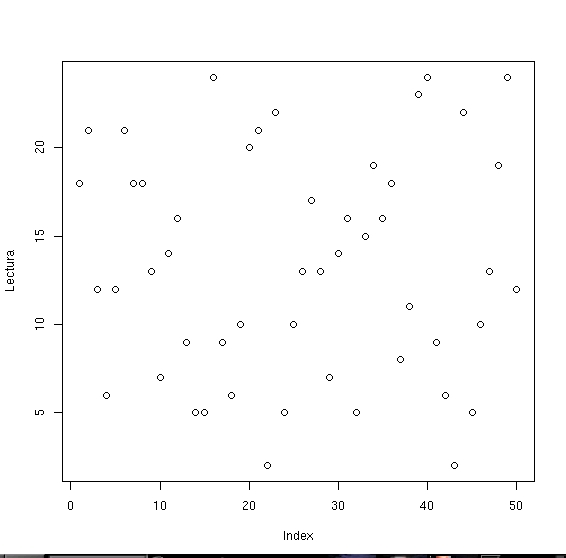
\includegraphics[width=0.49\textwidth]{imagenes/r_plot_1.eps}}
\subfigure[{\tt plot (Lectura, TV)}]{%
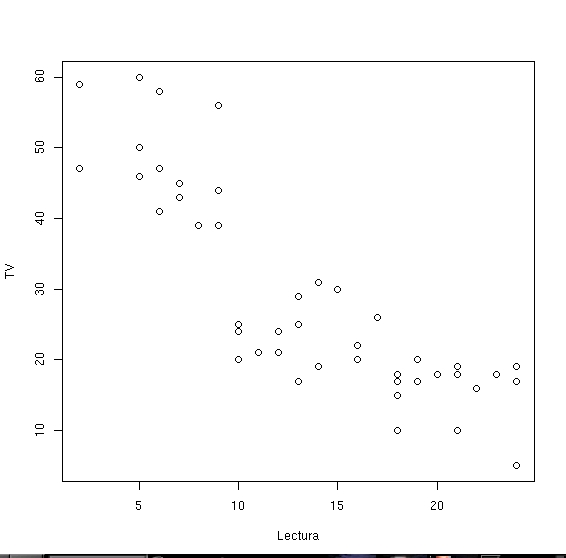
\includegraphics[width=0.49\textwidth]{imagenes/r_plot_2.eps}}
\subfigure[{\tt plot (Ingresos)}]{%
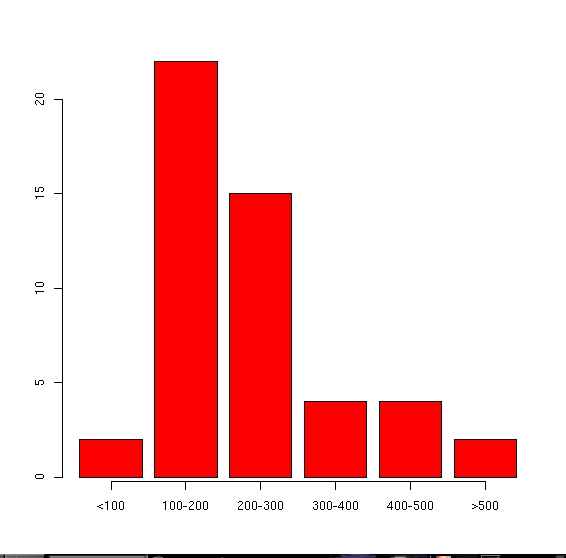
\includegraphics[width=0.49\textwidth]{imagenes/r_plot_3.eps}}
\subfigure[{\tt plot (Ingresos, Habitat)}]{%
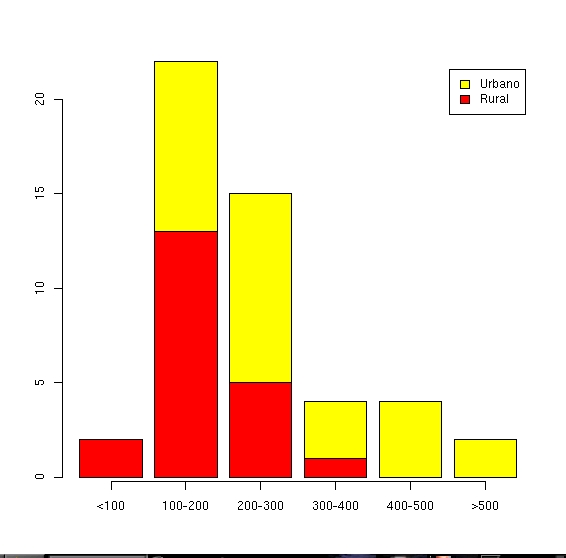
\includegraphics[width=0.49\textwidth]{imagenes/r_plot_4.eps}}
\caption{Las distintas formas de la función {\tt plot()}}
\end{figure}

\index{R!gráficas!qqplot@{\tt qqplot()}}

Otras gráficas interesantes son  las de comparación de distribuciones,
basadas en  los cuantiles. La función  {\tt qqnorm ()} toma  un vector
numérico y  lo representa comparando  sus cuantiles con  los cuantiles
teóricos  (los que  se  esperarían  en una  muestra  que siguiera  una
distribución normal). La función {\tt  qqline()} añade a la gráfica la
recta que pasa por los cuartiles de los datos y la distribución.

\begin{figure}[hbtp]
\centering
\subfigure[Gráfico Q-Q para {\tt Lectura}]{%
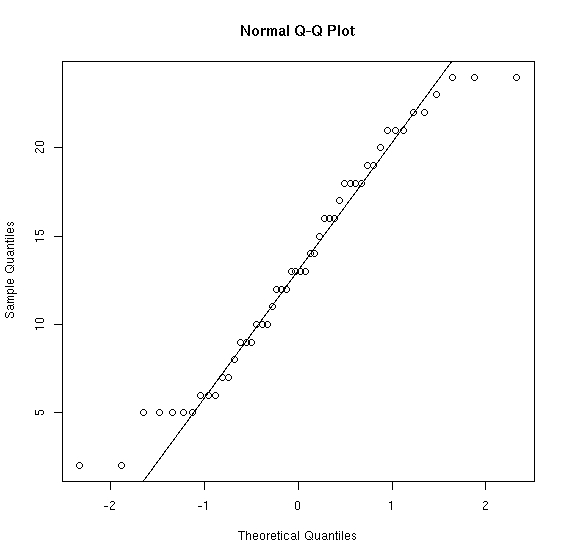
\includegraphics[width=0.49\textwidth]{imagenes/r_qqplot_1.eps}}
\subfigure[Gráfico Q-Q para {\tt TV}]{%
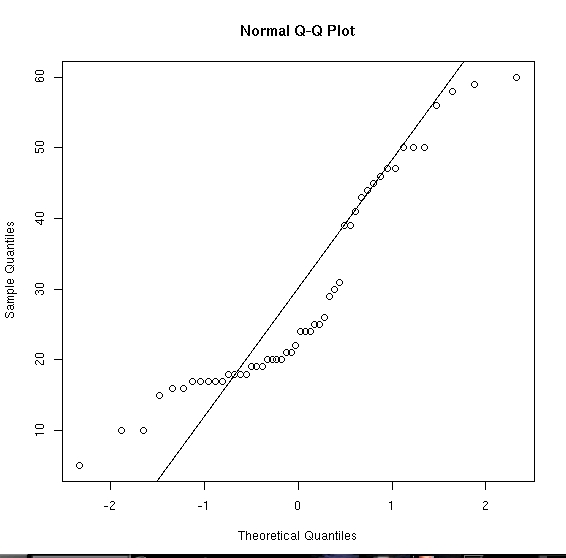
\includegraphics[width=0.49\textwidth]{imagenes/r_qqplot_2.eps}}
\caption[Gráficos Q-Q para dos variables]%
{Gráficos Q-Q para dos variables, una que se comporta como una
normal y otra que no}
\end{figure}

\index{R!gráficas!image@{\tt image()}}
\index{R!gráficas!contour@{\tt contour()}}
\index{R!gráficas!persp@{\tt persp()}}

Para  representar  matrices puedes  optar  por  ver sus  valores  como
imágenes. La  función {\tt image()} lo  hace a modo de  una rejilla de
rectángulos de  diferentes colores  para representar  el valor  de las
celdas. Para  verlo en forma de  contorno usa {\tt contour()},  y para
verlo en perspectiva utiliza {\tt persp()}.

\begin{figure}[htbp]
\centering
\subfigure[{\tt image(volcano)}]{%
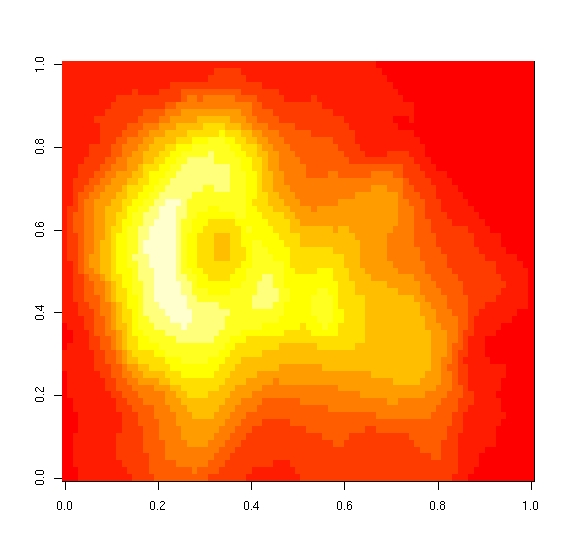
\includegraphics[width=0.49\textwidth]{imagenes/r_image.eps}}
\subfigure[{\tt contour(volcano)}]{%
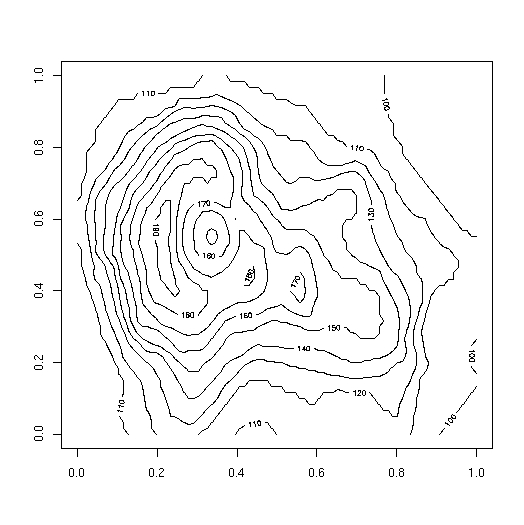
\includegraphics[width=0.49\textwidth]{imagenes/r_contour.eps}}
\subfigure[{\tt persp(volcano)}]{%
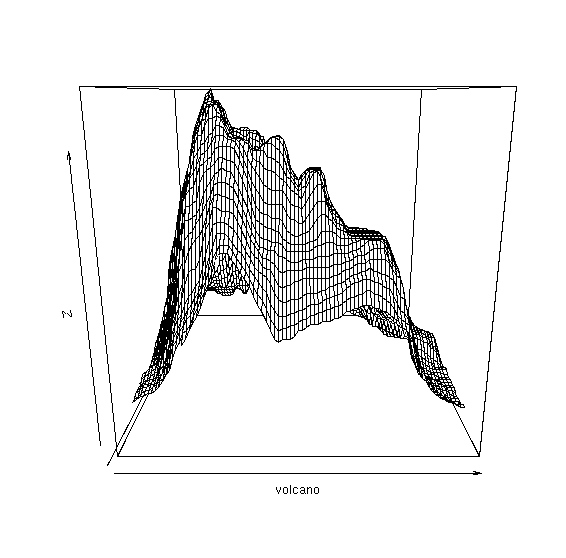
\includegraphics[width=0.49\textwidth]{imagenes/r_persp.eps}}
\subfigure[{\tt Gráfica de sectores para la Edad}]{%
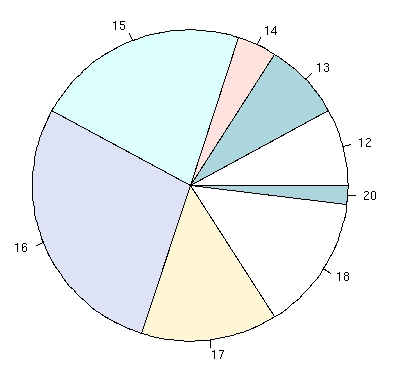
\includegraphics[width=0.49\textwidth]{imagenes/r_pie.eps}}
\caption[Gráficas para  representar matrices]%
{Gráficas para  representar matrices. El objeto  {\tt volcano}
lo obtenemos al ejecutar {\tt data(volcano)}}
\end{figure}

Los gráficos de sectores te dan una impresión clara a primera vista de
los  porcentajes que  tienen cada  ``clase'' en  una clasificación  de
datos.  Por ejemplo  para ver  los porcentajes  de personas  según las
edades representamos en un gráfico de sectores el número de individuos
que tiene cada edad. Una forma de hacerlo (seguramente no es la mejor)
sería:

\index{R!gráficas!de sectores}

\begin{verbatim}
> pie (tapply (Edad, fedad, length))
\end{verbatim}

\index{R!gráficas!pie@{\tt pie()}}
